
\begin{filecontents*}[overwrite]{refs.bib}
@inproceedings{jimenez2024swebench,
  author={Jimenez, Carlos E. and Yang, John and Wettig, Alexander and Yao, Shunyu and Pei, Kexin and Press, Ofir and Narasimhan, Karthik},
  title={{SWE-bench}: Can Language Models Resolve Real-World {GitHub} Issues?},
  booktitle={International Conference on Learning Representations (ICLR)}, year={2024},
  doi={10.48550/arXiv.2310.06770}}
@inproceedings{yang2024sweagent,
  author={Yang, John and Jimenez, Carlos E. and Wettig, Alexander and Lieret, Kilian and Yao, Shunyu and Narasimhan, Karthik and Press, Ofir},
  title={{SWE-agent}: Agent-Computer Interfaces Enable Automated Software Engineering},
  booktitle={Advances in Neural Information Processing Systems (NeurIPS)}, year={2024},
  doi={10.48550/arXiv.2405.15793}}
@inproceedings{jain2025livecodebench,
  author={Jain, Naman and Han, King and Gu, Alex and Li, Wen-Ding and Yan, Fanjia and Zhang, Tianjun and Wang, Sida and Solar-Lezama, Armando and Sen, Koushik and Stoica, Ion},
  title={{LiveCodeBench}: Holistic and Contamination Free Evaluation of Large Language Models for Code},
  booktitle={International Conference on Learning Representations (ICLR)}, year={2025},
  doi={10.48550/arXiv.2403.07974}}
@article{chen2021humaneval,
  author={Chen, Mark and Tworek, Jerry and Jun, Heewoo and Yuan, Qiming and others},
  title={Evaluating Large Language Models Trained on Code}, journal={arXiv preprint arXiv:2107.03374}, year={2021},
  doi={10.48550/arXiv.2107.03374}}
@inproceedings{jiang2023llmlingua,
  author={Jiang, Huiqiang and Wu, Qianhui and Lin, Chin-Yew and Yang, Yuqing and Qiu, Lili},
  title={{LLMLingua}: Compressing Prompts for Accelerated Inference of Large Language Models},
  booktitle={Conference on Empirical Methods in Natural Language Processing (EMNLP)}, year={2023}, note={arXiv:2310.05736},
  doi={10.18653/v1/2023.emnlp-main.825}}
@inproceedings{zheng2024sglang,
  author={Zheng, Lianmin and Yin, Liangsheng and Xie, Zhiqiang and others},
  title={{SGLang}: Efficient Execution of Structured Language Model Programs},
  booktitle={Advances in Neural Information Processing Systems (NeurIPS)}, year={2024},
  doi={10.48550/arXiv.2312.07104}}
@article{chen2023frugalgpt,
  author={Chen, Lingjiao and Zaharia, Matei and Zou, James},
  title={{FrugalGPT}: How to Use Large Language Models While Reducing Cost and Improving Performance},
  journal={arXiv preprint arXiv:2305.05176}, year={2023}, doi={10.48550/arXiv.2305.05176}}
@article{schwartz2020greenai,
  author={Schwartz, Roy and Dodge, Jesse and Smith, Noah A. and Etzioni, Oren},
  title={Green {AI}}, journal={Communications of the ACM}, volume={63}, number={12}, pages={54--63}, year={2020},
  doi={10.1145/3381831}}
@inproceedings{raji2021benchmark,
  author={Raji, Inioluwa Deborah and Denton, Emily and Bender, Emily M. and Hanna, Alex and Paullada, Amandalynne},
  title={{AI} and the Everything in the Whole Wide World Benchmark},
  booktitle={NeurIPS Datasets and Benchmarks Track}, year={2021},
  doi={10.48550/arXiv.2111.15366}}
@article{biderman2024lessons,
  author={Biderman, Stella and Schoelkopf, Hailey and Sutawika, Lintang and Gao, Leo and Tow, Jonathan and others},
  title={Lessons from the Trenches on Reproducible Evaluation of Language Models},
  journal={arXiv preprint arXiv:2405.14782}, year={2024}, doi={10.48550/arXiv.2405.14782}}
@inproceedings{jacobs2021measurement,
  author={Jacobs, Abigail Z. and Wallach, Hanna},
  title={Measurement and Fairness},
  booktitle={ACM Conference on Fairness, Accountability, and Transparency (FAccT)}, pages={375--385}, year={2021},
  doi={10.1145/3442188.3445901}}
@inproceedings{yao2023react,
  author={Yao, Shunyu and Zhao, Jeffrey and Yu, Dian and Du, Nan and Shafran, Izhak and Narasimhan, Karthik and Cao, Yuan},
  title={{ReAct}: Synergizing Reasoning and Acting in Language Models},
  booktitle={International Conference on Learning Representations (ICLR)}, year={2023},
  doi={10.48550/arXiv.2210.03629}}
@inproceedings{schick2023toolformer,
  author={Schick, Timo and Dwivedi-Yu, Jane and Dess{\`i}, Roberto and Raileanu, Roberta and Lomeli, Maria and Hambro, Eric and Zettlemoyer, Luke and Cancedda, Nicola and Scialom, Thomas},
  title={{Toolformer}: Language Models Can Teach Themselves to Use Tools},
  booktitle={Advances in Neural Information Processing Systems (NeurIPS)}, year={2023},
  doi={10.48550/arXiv.2302.04761}}
@article{liu2024seagentsurvey,
  author={Liu, Junwei and Wang, Kaixin and Chen, Yixuan and Peng, Xin and Chen, Zhenpeng and Zhang, Lingming and Lou, Yiling},
  title={Large Language Model-Based Agents for Software Engineering: A Survey},
  journal={arXiv preprint arXiv:2409.02977}, year={2024}, doi={10.48550/arXiv.2409.02977}}
@inproceedings{agarwal2021precipice,
  author={Agarwal, Rishabh and Schwarzer, Max and Castro, Pablo Samuel and Courville, Aaron and Bellemare, Marc G.},
  title={Deep Reinforcement Learning at the Edge of the Statistical Precipice},
  booktitle={Advances in Neural Information Processing Systems (NeurIPS)}, year={2021},
  doi={10.48550/arXiv.2108.13264}}
@article{liang2023helm,
  author={Liang, Percy and Bommasani, Rishi and Lee, Tony and others},
  title={Holistic Evaluation of Language Models}, journal={Transactions on Machine Learning Research (TMLR)}, year={2023},
  doi={10.48550/arXiv.2211.09110}}
@article{kapoor2024agentsmatter,
  author={Kapoor, Sayash and Stroebl, Benedikt and Siegel, Zachary S. and Nadgir, Nitya and Narayanan, Arvind},
  title={{AI} Agents That Matter}, journal={arXiv preprint arXiv:2407.01502}, year={2024},
  doi={10.48550/arXiv.2407.01502}}
@inproceedings{dehghani2022efficiency,
  author={Dehghani, Mostafa and Tay, Yi and Arnab, Anurag and Beyer, Lucas and Vaswani, Ashish},
  title={The Efficiency Misnomer},
  booktitle={International Conference on Learning Representations (ICLR)}, year={2022},
  doi={10.48550/arXiv.2110.12894}}
@article{barke2023grounded,
  author={Barke, Shraddha and James, Michael B. and Polikarpova, Nadia},
  title={Grounded {Copilot}: How Programmers Interact with Code-Generating Models},
  journal={Proceedings of the ACM on Programming Languages (OOPSLA)}, volume={7}, pages={85--111}, year={2023},
  doi={10.1145/3586030}}
@article{bai2026spend,
  author={Bai, Longju and Huang, Zhemin and Wang, Xingyao and Sun, Jiao and Mihalcea, Rada and Brynjolfsson, Erik and Pentland, Alex and Pei, Jiaxin},
  title={How Do {AI} Agents Spend Your Money? Analyzing and Predicting Token Consumption in Agentic Coding Tasks},
  journal={arXiv preprint arXiv:2604.22750}, year={2026}, doi={10.48550/arXiv.2604.22750}}
@misc{jetbrains2026caveman,
  author={Shiryaev, Denis},
  title={Does Speaking to Agents Like Cavemen Really Save 65\% of Tokens? {We} Test},
  year={2026},
  howpublished={{JetBrains} {AI} blog},
  url={https://blog.jetbrains.com/ai/2026/07/speak-to-ai-agents-like-cavemen-tosave-tokens/},
  note={Independent A/B test of the caveman skill on 86 {Claude Code} tasks; about 8.5\% output savings vs.\ the advertised 65\%. Secondary coverage: \url{https://www.infoworld.com/article/4193775/talk-like-a-caveman-prompts-save-tokens-but-far-less-than-promised.html}}}
@inproceedings{lago2024threats,
  author={Lago, Patricia and Runeson, Per and Song, Qunying and Verdecchia, Roberto},
  title={Threats to Validity in Software Engineering -- hypocritical paper section or essential analysis?},
  booktitle={Proceedings of the 18th ACM/IEEE International Symposium on Empirical Software Engineering and Measurement (ESEM)},
  pages={314--324}, year={2024}, doi={10.1145/3674805.3686691}}
@article{erol2025costofpass,
  author={Erol, Mehmet Hamza and El, Batu and Suzgun, Mirac and Yuksekgonul, Mert and Zou, James},
  title={Cost-of-Pass: An Economic Framework for Evaluating Language Models},
  journal={arXiv preprint arXiv:2504.13359}, year={2025}, doi={10.48550/arXiv.2504.13359}}
@inproceedings{bean2025construct,
  author={Bean, Andrew M. and Kearns, Ryan Othniel and Romanou, Angelika and others},
  title={Measuring What Matters: Construct Validity in Large Language Model Benchmarks},
  booktitle={NeurIPS Datasets and Benchmarks Track}, year={2025},
  doi={10.48550/arXiv.2511.04703}}
@inproceedings{liu2023evalplus,
  author={Liu, Jiawei and Xia, Chunqiu Steven and Wang, Yuyao and Zhang, Lingming},
  title={Is Your Code Generated by {ChatGPT} Really Correct? Rigorous Evaluation of Large Language Models for Code Generation},
  booktitle={Advances in Neural Information Processing Systems (NeurIPS)}, year={2023},
  doi={10.48550/arXiv.2305.01210}}
@article{liang2025swebenchillusion,
  author={Liang, Shanchao and Garg, Spandan and Zilouchian Moghaddam, Roshanak},
  title={The {SWE-Bench} Illusion: When State-of-the-Art {LLMs} Remember Instead of Reason},
  journal={arXiv preprint arXiv:2506.12286}, year={2025}, doi={10.48550/arXiv.2506.12286}}
@article{yao2024taubench,
  author={Yao, Shunyu and Shinn, Noah and Razavi, Pedram and Narasimhan, Karthik},
  title={{$\tau$-bench}: A Benchmark for Tool-Agent-User Interaction in Real-World Domains},
  journal={arXiv preprint arXiv:2406.12045}, year={2024}, doi={10.48550/arXiv.2406.12045}}
\end{filecontents*}

\documentclass[sigconf,screen]{acmart}

\IfFileExists{libertine.sty}{}{%
  \PackageError{paper}{libertine is missing on this machine - the PDF would be typeset in Computer
  Modern and would not meet the ACM font requirement. Build in the texlive container instead}{}}
\setcopyright{cc}
\setcctype{by}
\acmDOI{10.1145/3843282.3844423}
\acmYear{2026}
\copyrightyear{2026}
\acmISBN{979-8-4007-2985-0/2026/10}
\acmConference[AgenticDev '26]{Proceedings of the 1st International Workshop on Agentic AI for Next-Generation Software Development}{October 12--16, 2026}{Munich, Germany}
\acmBooktitle{Proceedings of the 1st International Workshop on Agentic AI for Next-Generation Software Development (AgenticDev '26), October 12--16, 2026, Munich, Germany}
\acmSubmissionID{asews26agenticdevmain-p20-p}
\received{2026-07-22}
\received[accepted]{2026-08-20}
\microtypesetup{expansion=false}

\makeatletter
\def\venuetextblockw{7.087}
\def\venuetextblockh{9.252}
\def\venuecolumns{2}
\def\venuebodypt{9}
\def\venuebodypagesmax{5}
\def\venuerefpagesmax{2}

\let\paper@bibliography\bibliography
\renewcommand{\bibliography}[1]{\label{paper@bodyend}\paper@bibliography{#1}}
\def\paper@page#1#2#3\@nil{#2}
\AtEndDocument{{\normalsize\xdef\paper@bodysize{\f@size}}%
  \ifnum\venuecolumns=2\relax
    \if@twocolumn\else\PackageError{paper}{one-column output, venue requires \venuecolumns}{}\fi
  \else\if@twocolumn\PackageError{paper}{two-column output, venue requires \venuecolumns}{}\fi\fi
  \ifdim\textwidth>\venuetextblockw in\relax
    \PackageError{paper}{textwidth \the\textwidth exceeds venue max \venuetextblockw in}{}\fi
  \ifdim\textheight>\venuetextblockh in\relax
    \PackageError{paper}{textheight \the\textheight exceeds venue max \venuetextblockh in}{}\fi
  \ifdim\paper@bodysize pt=\venuebodypt pt\relax\else
    \PackageError{paper}{body font \paper@bodysize pt, venue requires \venuebodypt pt}{}\fi
  \@ifundefined{r@paper@bodyend}{}{%
    \edef\paper@be{\expandafter\expandafter\expandafter
      \paper@page\csname r@paper@bodyend\endcsname\@nil}%
    \ifnum\paper@be>\venuebodypagesmax\relax
      \PackageError{paper}{body ends on page \paper@be, venue limit \venuebodypagesmax}{}\fi
    \@tempcnta=\value{page}\advance\@tempcnta-\paper@be\relax
        \ifnum\@tempcnta>\venuerefpagesmax\relax
      \PackageError{paper}{references use \the\@tempcnta extra page(s), venue allows \venuerefpagesmax}{}\fi}%
  \typeout{GUARDPROBE bodyend=\@ifundefined{r@paper@bodyend}{NONE}{\paper@be} last=\the\value{page}}%
  \ifdefined\finalpass
    \ifx\@refundefined\relax\else
      \PackageError{paper}{undefined references - see the log}{}\fi
    \@ifundefined{NAT@undefined}{}{%
      \PackageError{paper}{undefined citations (natbib) - see the log}{}}%
  \fi
}
\makeatother

\usepackage{tikz}
\usepackage{xurl}
\setlength{\emergencystretch}{3em}

\begin{document}

\title[Measuring the Wrong Number: Cost-Aware, Correctness-Gated Evaluation \ldots]{Measuring the Wrong Number: Cost-Aware, Correctness-Gated Evaluation of Efficiency Claims in Multi-turn Agentic Coding}

\author{Erdni Zergetaev}
\affiliation{%
  \institution{Independent Researcher}
  \city{Almaty}
  \country{Kazakhstan}}
\email{zergetaev@gmail.com}

\begin{abstract}
A fast-growing ecosystem of plugins, skills, and prompt packs promises to make AI coding agents
cheaper. The most popular single artifact---a ``talk-like-a-caveman'' skill for a widely used coding
agent---has ${\sim}92{,}000$ GitHub stars (as of 2026-07) and advertises a 65\% token reduction. We show that such
claims, though not fabricated, \emph{measure the wrong number}. Efficiency tools are validated on
single-shot question answering and report \textbf{output-token} reduction, whereas a real agentic
coding session is dominated by \textbf{input and cached context} re-read every turn; the model's own
output is only ${\approx}0.6\%$ of session tokens in aggregate and ${\approx}20\%$ of the dollar cost. We
introduce a reproducible, \textbf{cost-aware, correctness-gated} A/B harness that installs each tool
faithfully, runs repeated trials over multi-turn coding tasks, breaks the bill down by token
class, and gates every trial on a structural correctness check. Across 140 runs on two widely used efficiency
tools --- the two most-starred in this category --- neither the token claim nor the money behind it
survives. Output falls far short of the advertised 63--75\%, which an industry test had already
found; the finding we add is that the \textbf{dollar bill does not move at all}, coming out
statistically flat with confidence intervals that exclude any saving close to the advertised
figures. The ceiling is also structural: output is only
about a fifth of the bill, so even a \emph{perfect} 65\% output cut caps bill savings near ${\approx}13\%$. We argue that trustworthy evaluation of agent tooling must
measure cost on realistic multi-turn sessions with a correctness gate, and we release the recorded
measurements with a self-checking script that reproduces every number.
\end{abstract}

\begin{CCSXML}
<ccs2012>
   <concept>
       <concept_id>10011007.10011074.10011099</concept_id>
       <concept_desc>Software and its engineering~Software verification and validation</concept_desc>
       <concept_significance>500</concept_significance>
       </concept>
   <concept>
       <concept_id>10002944.10011123.10010912</concept_id>
       <concept_desc>General and reference~Empirical studies</concept_desc>
       <concept_significance>300</concept_significance>
       </concept>
   <concept>
       <concept_id>10010147.10010178.10010179</concept_id>
       <concept_desc>Computing methodologies~Natural language processing</concept_desc>
       <concept_significance>100</concept_significance>
       </concept>
 </ccs2012>
\end{CCSXML}

\ccsdesc[500]{Software and its engineering~Software verification and validation}
\ccsdesc[300]{General and reference~Empirical studies}
\ccsdesc[100]{Computing methodologies~Natural language processing}

\keywords{AI coding agents, LLM tooling, evaluation, benchmarking, cost, reproducibility}

\maketitle

\section{Introduction}
\label{sec:intro}
AI coding agents and their open harnesses~\cite{yang2024sweagent} are increasingly configured with
third-party \emph{plugins, skills, and hooks} that claim to improve cost, speed, or safety. Built on
the reasoning-and-acting loops that define modern agents~\cite{yao2023react,schick2023toolformer},
these tools spread virally---stars, roundups, social posts---far faster than they are independently
validated. Assistants of this kind are already woven into how programmers work day to
day~\cite{barke2023grounded}. An \textbf{unverified performance claim} about one of them therefore does
not stay on a README; it propagates into practice. While the
community has invested heavily in evaluating agent
\emph{capability}~\cite{jimenez2024swebench,jain2025livecodebench,liu2024seagentsurvey},
the \emph{cost} claims of the surrounding tooling are largely taken on trust.

We focus on the most visible category: \textbf{token-efficiency} tools. The flagship example is a
skill that instructs the model to answer in terse, telegraphic prose (``caveman mode''); its
description advertises ``${\sim}75\%$'' and its README ``65\%'' token savings, and as of
2026-07 it carries ${\sim}92{,}000$ GitHub
stars.\footnote{\url{https://github.com/juliusbrussee/caveman}} A second popular tool ships a compact
project-memory file and advertises a ``63\%'' reduction (\textbf{Token-Eff.}\ in the
tables).\footnote{\url{https://github.com/drona23/claude-token-efficient}} We measured
\texttt{caveman@f06348c} and \texttt{claude-token-efficient@0d30a6d}, fetched on 2026-06-20 and
2026-06-21 and vendored into the released harness. Naming the commits matters more than usual here:
both projects move fast --- the first went from 75k to 92k stars over the weeks around our runs ---
so a reader checking later is otherwise testing a different tool than we did.

Two separate claims are bundled inside that headline, and they fail for different reasons. The first
is that the tool cuts output tokens by 65\%. That one has already been questioned: an industry A/B
test over 86 coding tasks measured about 8.5\% output savings~\cite{jetbrains2026caveman}, and our
runs agree at about 6\%. The second claim is the one users actually care about---that trimming output
shrinks the bill by a comparable amount. Nobody had measured it. It fails for a reason independent of
the first: output is only about a fifth of what a coding session costs, so even an honest 65\% cut
could not move the bill by 65\%. This paper is about the second claim, the one that decides what a user pays.

\textbf{RQ: when a token-efficiency tool is installed the
way a user installs it and run on multi-turn coding work, how much does the dollar bill actually
change, and what bounds that change?} The first half is measured, the second is derived from the cost
structure, and the second explains why nothing larger was available to find.

Our contribution is not that ``input dominates output''---recent work measures token consumption
across frontier models and finds input, not output, drives agentic cost~\cite{bai2026spend}---but a
\emph{measurement method} aimed at \emph{third-party tools' advertised claims}, and the evidence it produces:
\begin{enumerate}
  \item We identify \textbf{why} the headline claims are systematically inflated: they are produced
  on single-shot Q\&A, count output tokens only, and use a no-concision baseline, none of which
  describe how a coding agent actually runs (Section~\ref{sec:pitfall}).
  \item We build a \textbf{cost-aware, correctness-gated} A/B harness that installs each tool the way
  a user would, runs repeated multi-turn trials, breaks the bill down by token class, and rejects any
  trial that regresses correctness (Section~\ref{sec:method}).
  \item We measure two widely used tools across 140 runs. Output falls far short of the advertised
  figures, which confirms~\cite{jetbrains2026caveman} on an independent harness. The \textbf{dollar
  bill does not move at all}, which is the new result, and a \textbf{structural bound} explains why no
  output-trimming tool can move it much (Section~\ref{sec:results}).
\end{enumerate}
The broader point is about trust in agent tooling: an advertised number is only meaningful under
the conditions its consumers face, or it misleads~\cite{raji2021benchmark,jacobs2021measurement}.

\section{The measurement pitfall}
\label{sec:pitfall}
\textbf{Three token classes, three prices.} A modern agent bills tokens at sharply different rates:
generated \textbf{output} is the most expensive; \textbf{input} you send is cheaper; and
\textbf{cached context} re-read each turn is cheapest of all (on the model we test, output is priced
${\approx}5\times$ input and ${\approx}50\times$ cache-read). A multi-turn agentic
session~\cite{yang2024sweagent} re-reads the entire conversation---files, tool results, prior
turns---on every step; prefix caching~\cite{zheng2024sglang} makes this cheap per token but there is
an enormous amount of it, so cached input dominates the volume and the model's fresh output is a
sliver.

\textbf{Why the headline numbers inflate.} Reading the upstream benchmark code that generates the
advertised figures, we find four choices, each the \emph{opposite} of how a coding agent actually runs: (i)
\textbf{single-shot, one-turn Q\&A}---one user message, no tools, no file reads; (ii) \textbf{output
tokens only}---input (including the tool's own always-loaded prompt) is never counted; (iii) a
\textbf{no-concision baseline} (``You are a helpful assistant.''), so the tool beats a rambler; and
(iv) \textbf{no correctness gate}---terser answers count as savings even if they drop information.
The reported number measures something other than what it claims
to~\cite{raji2021benchmark,jacobs2021measurement}: the advertised quantity is not the one the user
cares about. The fix is to measure \textbf{dollar cost on multi-turn sessions with a correctness
gate}, as cost-focused evaluation work urges~\cite{chen2023frugalgpt,liang2023helm,schwartz2020greenai},
rather than output-token counts on single prompts. The compression literature these tools imitate
targets \emph{input} prompts~\cite{jiang2023llmlingua}---the big slice; shaving output gets it backwards.

\section{Method: a cost-aware, correctness-gated harness}
\label{sec:method}
The harness --- the ecosystem benchmark in \textsc{vigiles}, our open-source auditor for agent
harnesses --- is a reusable instrument rather than a
one-off script for this study: it A/B-tests any installable agent tool, and the two we report are
simply its first subjects. We implement the evaluation as an A/B harness that runs each arm (with the tool installed, and
without) \emph{inside a production agentic harness}---\textbf{Claude Code} (the CLI coding agent), on Claude Sonnet---rather than issuing isolated
API calls, so tools load and act exactly as they do for a real user; the harness is released as open
source. Figure~\ref{fig:harness} shows the whole path a task takes through it; its design choices
target the pitfalls of Section~\ref{sec:pitfall}.

\begin{figure}[t]
\centering
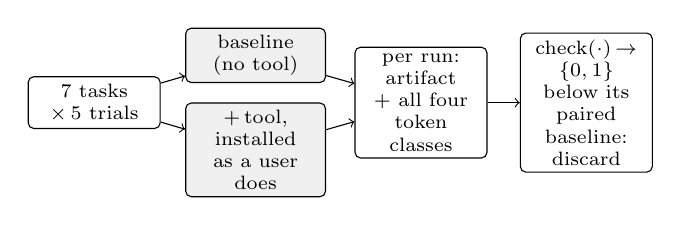
\begin{tikzpicture}[
  font=\scriptsize,
  b/.style={draw, rounded corners=2pt, align=center, inner sep=2.5pt, text width=1.5cm},
  s/.style={draw, rounded corners=2pt, align=center, inner sep=2.5pt, text width=1.6cm, fill=black!6}
]
  \node[b] (t)  at (0,0)      {7 tasks\\$\times$\,5 trials};
  \node[s] (a)  at (2.05,0.6) {baseline\\(no tool)};
  \node[s] (k)  at (2.05,-0.6){$+$\,tool, installed\\as a user does};
  \node[b] (r)  at (4.15,0)   {per run: artifact\\$+$ all four\\token classes};
  \node[b] (g)  at (6.25,0)   {check$(\cdot)\!\to\!\{0,1\}$\\below its paired\\baseline: discard};
  \draw[->] (t) -- (a);   \draw[->] (t) -- (k);
  \draw[->] (a) -- (r);   \draw[->] (k) -- (r);
  \draw[->] (r) -- (g);
\end{tikzpicture}
\caption{The harness. Each task is run both ways, five times each, inside the real agent. Two things
make it different from how efficiency tools are usually measured: the tool is installed the way a user
installs it (a file merely dropped in the directory never loads), and every run is priced across
\emph{all four} token classes---input, cache-read, cache-write, output---not just the one the tool
advertises. Runs that lose correctness against their own baseline are thrown out before any saving is
counted.}
\Description{A left-to-right flow diagram of the experimental harness. On the left, a box reading
``7 tasks times 5 trials'' branches into two shaded boxes stacked vertically: a baseline arm with no
tool, and a second arm with the tool installed the way a user installs it. Both arms feed into a box
recording, for every run, the produced artifact together with all four token classes. That box feeds
a final gate box: a deterministic check returning zero or one, where a run scoring below its own
paired baseline is discarded.}
\label{fig:harness}
\end{figure}

\textbf{Faithful installation.} Each tool is delivered \emph{as a user installs it} --- the
install step that decides whether a tool has any effect at all. A
skill that ships as a plugin is loaded via the agent's real plugin mechanism together with its own
activation hook, so it is active from the first message; a tool that ships as project memory is placed
where the agent auto-loads it. This step is load-bearing: a bare skill file merely dropped in the working
directory never registers and silently no-ops, which invalidated an earlier run until we caught
it~\cite{biderman2024lessons}.

\textbf{Repeated, multi-turn tasks.} We use seven self-contained coding tasks
(Table~\ref{tab:tasks} gives each one, what it must produce, and what its check asserts) --- from
one-line helpers (\texttt{slugify}, \texttt{debounce}), through an off-by-one bugfix and a regex
task, to a documentation review and a multi-file \texttt{refactor-suite}. The suite deliberately skews
short (each task runs ${\le}10$ turns), a limitation we return to in Section~\ref{sec:threats}; even so,
output is already a sliver, and longer sessions only shrink its share. Each task is run with the
tool (``skill'' arm) and without (``baseline'' arm), five trials per arm (repeated trials for
reliability~\cite{yao2024taubench}), on Claude Sonnet,
for $7\text{ tasks}\times5\text{ trials}\times2\text{ arms}\times2\text{ tools} = 140$ runs. The runs date
from July 2026 and name the model by the vendor's \texttt{sonnet} alias, which resolves to whichever
build the installed agent defaults to; we did not pin an exact one, so a later replication is running
a nearby model rather than the same one. The two
tools are the caveman skill and \textbf{Token-Eff.}, introduced in Section~\ref{sec:intro}; that total
describes our study, and a user evaluating a single tool would run half of it.

\begin{table}[t]
\centering
\caption{The seven tasks. Every trial must pass the check in the right-hand column; a skill-arm trial
scoring below its paired baseline is discarded. Checks are structural rather than full execution, a
shallowness we treat as a threat in Section~\ref{sec:threats}. The exact assertions ship with the harness.}
\label{tab:tasks}
\small
\setlength{\tabcolsep}{3pt}
\begin{tabular}{@{}lp{2.3cm}p{3.4cm}@{}}
\toprule
Task & Must produce & Check asserts \\
\midrule
\texttt{slugify} & \texttt{slugify(s)} + prose & defines it, uses \texttt{toLowerCase} and \texttt{replace} \\
\texttt{debounce} & \texttt{debounce(fn,ms)} + prose & contains \texttt{setTimeout} and \texttt{clearTimeout} \\
\texttt{bugfix-offbyone} & corrected \texttt{lastN} + prose & starts at \texttt{length-n}, not \texttt{length-n-1} \\
\texttt{bigO} & complexity + prose & final line states quadratic \\
\texttt{regex-email} & \texttt{isEmail(s)} + prose & defines it, requires \texttt{@}, uses a regex \\
\texttt{review-doc} & 3 files: cent-precision fix, review, bug name & \texttt{toFixed(0)} gone; review names two functions; bug named correctly \\
\texttt{refactor-suite} & 5 files across 3 modules: percentage fix, extracted helper, tests, review, bug name & flat-subtraction bug gone; helper exported once; tests present; review names the functions; bug named correctly \\
\bottomrule
\end{tabular}
\end{table}

\textbf{Whole-session cost breakdown.} For every run we record all token classes (input,
cache-read, cache-write, output) and price them at published API list rates (2026-08), reporting the \textbf{dollar
cost}~\cite{chen2023frugalgpt,schwartz2020greenai}, not a token count. On a subscription the ``bill''
is a usage quota with an opaque weighting, but that weighting must sit somewhere between raw token
counts (output ${\approx}0.6\%$) and API prices (output ${\approx}20\%$). We report dollars---the
weighting \emph{most} favorable to the tools; under any other, the ceiling only drops.

\textbf{Correctness gate.} Each task carries a \emph{deterministic structural}
$\textsf{check}(\cdot)\rightarrow\{0,1\}$ on the produced artifact --- e.g.\ the string-slug task must
define the function and use the right string operations, the off-by-one bugfix must actually move the
boundary condition, and the complexity task must state the correct big-O (the exact per-task assertions
are in the released harness).
These are lightweight structural checks rather than full execution as in HumanEval/SWE-bench~\cite{chen2021humaneval,jimenez2024swebench};
we keep their correctness-first discipline but check less deeply, and Section~\ref{sec:threats} treats that
shallowness as an explicit threat. A trial where the skill arm scores lower than its paired
baseline is a \emph{regression} and disqualifies the run, guarding against ``savings'' that are really
information loss (the gate is shallow and, as it happens, never fired --- Section~\ref{sec:threats}).

\textbf{Statistics.} For each task we report the mean change in output and a Welch $t$-test (a standard
test for whether two averages differ). We call an effect significant at $p<0.05$. We also note which
effects survive a Bonferroni correction: a stricter bar that guards against false positives when seven
tests are run at once, applied \emph{within} each tool. For the bill we report the pooled-dollar change
(total dollars across all tasks) and a paired $t$-test on the seven per-task cost differences, with a
95\% CI\@. Averages taken over a few trials are unreliable~\cite{agarwal2021precipice}, so we treat the
per-task spread as a result in its own right and report it rather than averaging it away.

This protocol is sized to \emph{audit} a public claim; adopting one tool needs far less --- your own
tasks, one tool, the total dollars across them. Two things are still required either way: the
correctness gate and the per-token-class breakdown.

\section{Results}
\label{sec:results}
\subsection{The advertised savings don't show up}
The flagship skill (claim 65\%)
delivers a \textbf{mean output cut of ${\approx}6\%$} (Table~\ref{tab:pertask}), with two per-task cuts that are individually
significant and survive Bonferroni (bugfix $-31\%$, $p{=}0.002$; regex $-28\%$, $p{=}0.006$)---so it
genuinely compresses output---but it \emph{grows} output on two tasks, and the \textbf{dollar bill shows no saving near the
advertised magnitude}.

\emph{The bill barely moves for either tool.} We sign bill changes so positive means \emph{more expensive}. For
the flagship, the bill moves $-1\%$ pooled but $+5\%$ as an unweighted per-task average; the pooled
figure weights by dollars and is dominated by one costly task. Either way the answer is ``no
detectable change'': 95\% CI $[-21\%,+31\%]$, $p{\approx}0.66$, $n{=}7$. The second tool (claim 63\%) runs $+10\%$, with pooled and
per-task in agreement (95\% CI $[-8\%,+29\%]$, $p{\approx}0.22$). It is \textbf{also not significant}.
Its one per-task cell that clears $p<0.05$ is a cost \emph{increase}, not a saving (regex-email,
$+127\%$, $p{=}0.037$), and it does not survive the seven-task Bonferroni correction
($0.037\times7{\approx}0.26$). The intervals are wide: at $n{=}7$ they cannot resolve a saving below our
${\approx}13\%$ structural ceiling. But they \emph{exclude} anything near the advertised 63--75\%, and
both best estimates land at roughly zero. Whatever room remains is capped by the cost structure
described below.
\emph{Correctness.} Both arms passed the correctness gate on every run: \textbf{zero regressions on the checked properties}
(because the gate is a shallow check, this bounds information loss rather than proving output quality was fully
preserved; see Section~\ref{sec:threats}).

\emph{A hidden penalty on short tasks.} A sharper signal hides in the token classes: on the shortest
tasks a tool's own always-loaded prompt can \emph{add} more cached input than it removes in output ---
the flagship's \texttt{slugify} arm carried ${\sim}70\%$ more cached tokens and cost ${\sim}66\%$ more
than baseline --- the opposite of an efficiency win. This is a short-session effect that amortizes
away; Section~\ref{sec:threats} narrows it.

\begin{table}[t]
\caption{Per-task output change (negative $=$ tool cut output), Welch $p$; \textbf{*} significant at
$0.05$ (uncorrected; see text for Bonferroni), n.s.${=}$not significant. Pooled dollar bill in the last row.}
\label{tab:pertask}
\small
\setlength{\tabcolsep}{4pt}
\resizebox{\columnwidth}{!}{%
\begin{tabular}{lrrrr}
\toprule
Task & Caveman $\Delta$Out & $p$ & Token-Eff. $\Delta$Out & $p$ \\
\midrule
slugify          & $+54\%$ & 0.27 & $-2\%$   & 0.78 \\
debounce         & $-28\%$ & 0.22 & $-7\%$   & 0.52 \\
bugfix-offbyone  & $\mathbf{-31\%}$ & \textbf{0.002*} & $-6\%$ & 0.87 \\
bigO             & $-18\%$ & 0.27 & $+6\%$   & 0.79 \\
regex-email      & $\mathbf{-28\%}$ & \textbf{0.006*} & $\mathbf{+127\%}$ & \textbf{0.037*} \\
review-doc       & $-8\%$  & 0.80 & $+54\%$  & 0.46 \\
refactor-suite   & $+21\%$ & 0.65 & $+33\%$  & 0.19 \\
\midrule
\textbf{bill} & \multicolumn{2}{l}{$\mathbf{-1\%}$ (n.s.)} & \multicolumn{2}{l}{$\mathbf{+10\%}$ (n.s.)} \\
\bottomrule
\end{tabular}%
}
\end{table}

\begin{figure}[t]
\centering
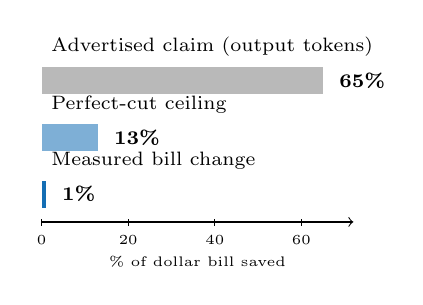
\begin{tikzpicture}[x=0.055cm,y=0.72cm]
  \definecolor{acc}{RGB}{20,110,180}
  \foreach \v/\lbl/\yy/\clr in {65/Advertised claim (output tokens)/2/gray!55, 13/Perfect-cut ceiling/1/acc!55, 1/Measured bill change/0/acc} {
    \node[anchor=south west, font=\scriptsize] at (0,\yy+0.5) {\lbl};
    \fill[\clr] (0,\yy) rectangle (\v,\yy+0.48);
    \node[anchor=west, font=\scriptsize\bfseries] at (\v+1.5,\yy+0.24) {\v\%};
  }
  \draw[->] (0,-0.25) -- (72,-0.25);
  \foreach \x in {0,20,40,60} { \draw (\x,-0.2) -- (\x,-0.32) node[anchor=north, font=\tiny] {\x}; }
  \node[anchor=north, font=\tiny] at (36,-0.68) {\% of dollar bill saved};
\end{tikzpicture}
\caption{The three different quantities. The advertised 65\% is an output-token reduction; because
output is only ${\approx}20\%$ of the dollar cost, even a \emph{perfect} 65\% cut caps bill savings at
${\approx}13\%$; the measured bill change for the flagship tool is ${\approx}0\%$ ($-1\%$ pooled; per-task
95\% CI $[-21\%,+31\%]$, n.s.). ``Measuring
the wrong number'' is the gap between the first bar and the third.}
\Description{A horizontal bar chart with three bars on a common axis running from zero to about
sixty-five percent. The top bar, the advertised saving, extends to sixty-five percent. The middle
bar, the ceiling that any output-only reduction can reach once output is priced as its true share of
the bill, extends to about thirteen percent. The bottom bar, the saving actually measured for the
flagship tool, is indistinguishable from zero.}
\label{fig:bound}
\end{figure}

\subsection{A ceiling for any output-trimming tool}
This is not a quirk of these two tools; it follows from the cost structure
(Figure~\ref{fig:bound}). Both shares below are \textbf{measured, not assumed}: we take the token counts
recorded in our own runs and divide the output charge by the dollar cost reported for the
same session. Pooled across all tasks and runs, output is \textbf{well under 1\% of session tokens}
(${\approx}0.6\%$ aggregate) and
\textbf{${\approx}20\%$ of the dollar cost}. If output is a fraction $f{\approx}0.20$ of the bill and
a tool removes a fraction $r$ of output, the bill falls by at most $f\cdot r$, assuming the session
itself (turns, tool calls, file reads) stays the same---and if it does not, the measured bills capture
that too. Even a \emph{perfect}
65\% output cut ($r{=}0.65$) caps bill savings at \textbf{${\approx}13\%$}---and neither tool
approaches $r{=}0.65$. The advertised 63--75\% and the achievable ${\le}13\%$ (at most ${\approx}18\%$ with cross-turn
compounding, Section~\ref{sec:threats}) are different
quantities; the claim optimizes the slice the user can see and leaves the ${\approx}80\%$ they cannot.
The flagship's other feature trims \emph{input} instead, and that route closes
too: it shrank an instructions file by 68\% but produced \textbf{no significant session saving}; a
few-hundred-token file is a rounding error against a ${\sim}100$k-token session.

\section{Discussion and threats to validity}
\label{sec:threats}
\textbf{What we claim.} Output is a small fraction of a real session (the bound's arithmetic
holds for any model, even where the exact share differs); the advertised output reductions do not
replicate at anything near their advertised size, and the compression that does survive does not
reproduce as a \emph{bill} reduction on multi-turn coding; the checked correctness properties never
regressed. We
measure \emph{cost}: latency and rate-limit headroom are different questions, which an output-side tool
might still improve; we do not evaluate them. We do \emph{not} claim ``these tools do nothing'' (the flagship measurably
compresses output) nor ``the bill always rises'' (its bill effect is flat/mixed). Nor do we dispute the
upstream output-token figures in their original single-shot setting. Our point is that they do not carry
over: once the setting changes to a multi-turn session, the number stops describing what the user pays.

\textbf{Threats.} We label each by its standard empirical category, so the section reports an analysis
rather than a ritual~\cite{lago2024threats}: whether the numbers support the inference (conclusion),
whether something other than the tool moved the bill (internal), how far the result carries
(external), and whether we measured the thing we name (construct).

\emph{Scale (conclusion).} We run five trials per task, so some per-task effects are dominated by
noise. That is itself part of the finding. Across tasks the flagship's output change ranges from a
$54\%$ growth to a $31\%$ cut (Table~\ref{tab:pertask})~\cite{agarwal2021precipice}. The honest
quantity is therefore a range straddling zero, never a clean 65\%. Our design refutes the advertised
\emph{magnitude}, but it cannot settle small bill differences (below ${\approx}13\%$) either way. What
caps those is the structural bound. A formal equivalence test (TOST---a test
for ``are these two effectively the same?'') on a larger corpus is future work. The harness is not
toothless, though: at $n{=}5$ it still detects per-task output cuts of
$28$--$31\%$ and a $66\%$ cost penalty. At that scale we read $p$-values as descriptive only,
and no conclusion rests on a single significance star.

\emph{Model (external).} We test one model, and cost \emph{ratios} vary by model. Anthropic's tiers all share a
5:1 output-to-input price ratio, so output's share of the bill is stable across them. The ceiling
scales linearly with that share. Even if output were priced twice as dearly, the cap on savings would
only rise to ${\approx}26\%$, still comfortably under half the advertised figure.

\emph{Task length (external).} Our tasks top out around ten turns. This cuts \emph{in our favor}. A longer session
re-reads a larger transcript on every turn, so output's share of tokens, and therefore of dollars, only
shrinks. That pushes the ${\le}13\%$ ceiling \emph{lower}, not higher. One might object that terser
output \emph{compounds}: each turn's output is re-read by every later turn, so trimming it early should
save more over a long session. But that downstream saving is billed at the cheap cache-read rate
(${\approx}50\times$ below output), and it scales only with output's small share of the re-read
transcript (a few percent). So it adds a few points at most. The compounded
ceiling is ${\approx}16$--$18\%$, still about a factor of ${\sim}4$ below the advertised figures. The
overhead runs the other way too. An always-loaded tool prompt adds a fixed cost every turn, which is
what drives the cost \emph{penalties} we see on the shortest tasks. That fixed cost amortizes over a
longer session, so those increases are themselves a short-session effect. The durable long-session
prediction is ``no change,'' not a penalty. An empirical long-session demonstration is still worthwhile
future work.

\emph{Attribution: harness vs.\ model (external).} Every run in the main study is Claude Code on Claude Sonnet, and those
are two separate limits worth separating. The \emph{harness} decides how many turns a task takes and
what is re-sent on each of them, so it, not the model, is what makes input dominate; the \emph{model}
mainly sets how wordy each reply is. A wordier model would raise the output share somewhat, but it
cannot stop the conversation and the files already read from being re-sent every turn, which is where
the asymmetry comes from. The ceiling of Section~\ref{sec:results} is arithmetic over whatever that
share turns out to be, so another agent moves the number and leaves the shape. A pilot on Claude
Haiku --- the cheapest model in the family, two tasks and two trials, far too few to quote an
effect --- puts output at $1.1\%$ of session tokens against the $0.6\%$ of the main study.
Nearly double, and still about one percent: the ceiling is recomputed from that share, not overturned
by it. Both runs ship in the released measurements.

A second harness is reachable but is not the same study run twice. The flagship now ships wrappers
for eight agents, OpenAI's Codex CLI among them, so the tool can be pointed at another harness; what
it delivers there differs, because that runtime rejects part of the loadout.\footnote{Wrapper list
and the rejected component are stated in the tool's own README as of 2026-08; the vendor's own
cross-harness benchmark nonetheless compares wrapped against direct \textbf{Claude Code}, so it too
stays inside one harness.} Measuring a second harness therefore compares two ecosystems, each with
its own installed capability, rather than drawing a second sample of this one --- worth doing, but it
answers a different question than the one asked here.

\emph{Multi-agent (external).} We do not study \emph{multi-agent} systems, where agents delegate to each
other: our unit is one agent using tools, which is what these artifacts are built for.

\emph{Generality (external).} We test two tools, and we wrote the tasks and checks ourselves (no external corpus).
The harness can A/B any installable tool, and extending the corpus is future work. The bias runs in our
favor: the suite skews \emph{short}, which if anything \emph{helps} an output-side tool show a saving,
and none did.

\emph{Cache dynamics (internal).} Our per-run bill uses the \emph{actual} token classes the API charged, not a
model of the cache, so cache writes and misses within a session are already priced in. A user can also
invalidate the cache at the session level: by editing the agent's memory file, adding a tool
server, or re-reading a changed file. (The first two rewrite the cached prefix, forcing everything after
it to be reprocessed.) All of these shift cost from cheap cache-reads toward input and cache-writes.
That is, they push cost \emph{further} toward context and away from output. They \emph{lower} the
${\le}13\%$ ceiling and cannot raise output's share. So our clean-caching tasks, if anything,
\emph{over}-state how much an output-side tool could ever save.

\emph{Gate shallowness (construct).} The correctness gate is a shallow check: it reads the answer for the right
shape without running the code. So ``zero regressions'' bounds gross information loss, but it does not
prove that the terser output kept every nuance a human reader would want. A stronger gate that runs the
code is future work. Still, a gate that never fires is doing real work: it rules out the reading that
the savings came from dropped content.
Without it, a harness would silently count information loss as ``savings.'' So the gate's silence is
itself a result: on the properties we checked, the tools' terseness did no damage.

\textbf{Implication.} The efficiency-claim failure is a special case of a general validation gap:
agent-tooling claims are routinely produced under conditions that do not match deployment. A
community norm of \textbf{cost-aware, correctness-gated, faithfully-installed} evaluation would let
practitioners adopt tools on evidence rather than stars.

\section{Related work}
\textbf{Evaluating coding agents.} Execution-based, correctness-gated benchmarks such as
HumanEval~\cite{chen2021humaneval}, SWE-bench~\cite{jimenez2024swebench}, and
LiveCodeBench~\cite{jain2025livecodebench}, together with agent interfaces like
SWE-agent~\cite{yang2024sweagent} and surveys of LLM agents for software
engineering~\cite{liu2024seagentsurvey}, evaluate \emph{capability} on real, multi-turn tasks. We
keep their correctness-first discipline but ask a question they leave open: what the session costs.

\textbf{Cost and efficiency.} Several lines of work push evaluation toward what things actually cost:
choosing models by cost~\cite{chen2023frugalgpt}, pricing the \emph{correct} solution rather than any
solution~\cite{erol2025costofpass}, scoring many metrics at once~\cite{liang2023helm}, treating
efficiency as a result in its own right~\cite{schwartz2020greenai}, compressing
prompts~\cite{jiang2023llmlingua}, and caching repeated context~\cite{zheng2024sglang}. We take the
same stance---price the whole session, in dollars---and our structural bound says why output-side
compression cannot move a session bill. Closest to us, \citet{kapoor2024agentsmatter} argue that agent
benchmarks must control for cost and that headline metrics mislead when it is ignored, and
\citet{dehghani2022efficiency} show that single efficiency metrics disagree with each other. We turn
that lens on \emph{third-party tooling claims}, and add faithful installation plus the output-share
bound: output is a small share of the bill, so cutting it can only save that share.
\citet{bai2026spend} profile token consumption at scale and confirm that input, not output, dominates
the bill---the fact we build on; what we add is the faithful-install audit of third-party tools'
\emph{advertised claims}.

\textbf{Measurement validity and reproducibility.} A long line of work shows that benchmarks often do
not measure what they claim~\cite{raji2021benchmark,jacobs2021measurement,bean2025construct}, that
evaluations are hard to reproduce~\cite{biderman2024lessons}, and that results from a handful of runs
need honest statistics~\cite{agarwal2021precipice}. \emph{Capability} benchmarks show the same failures
in other forms: weak tests that pass wrong code~\cite{liu2023evalplus}, and models that memorize
answers instead of reasoning~\cite{liang2025swebenchillusion}. We aim the same critique at a different
target: advertised \emph{cost} claims. The industry A/B test cited
above~\cite{jetbrains2026caveman} reached the same verdict on output volume, and its ${\approx}8.5\%$
is far short of the \emph{perfect} cut our ${\approx}13\%$ ceiling already assumes, so its effect on
the bill is smaller still. What we add over such informal measurements is a reproducible
harness---multi-turn, correctness-gated, with the bill broken down by token class---applied uniformly
to both tools, plus the audit of the upstream benchmark code and the structural bound.

\section{Conclusion}
The efficiency-tool market runs on a number that is not your bill. These tools trim what the model
says; you pay mostly for everything it had to read first. We measured two of the most popular ones
on real multi-turn sessions, installed the way a user installs them, with a correctness gate on
every run---and neither half of the claim survives: output falls far short of the
advertised 63--75\%, and the bill does not move at all.

The numbers are not fabricated; they are the wrong number. The output you are shown is only about a
fifth of what you pay for, and the ${\approx}80\%$ you cannot see is where the money goes: even a
\emph{perfect} 65\% output cut saves at most ${\approx}13\%$. Trimming the model's replies to shrink
your bill is like ordering a smaller dessert to shrink a dinner check; most of the check was never
the dessert.

We release the measurements with a self-checking script that reproduces every reported number, so
the next advertised claim can be re-run the same way. Before you
install the next efficiency plugin, ask which tokens it cuts---and whether anyone priced a real
session, not a one-line prompt.

\textbf{Availability.} The complete harness of Section~\ref{sec:method} and the seven task and check
definitions are public at \url{https://github.com/zernie/vigiles} under \path{bench/ecosystem/}. The
measurements are released per task and per arm ($n$, mean, standard deviation, standard error for
each token class), together with a self-checking script that re-derives every number reported here
and exits non-zero on any drift. Individual trial rows are not included: how much the runs of one task
varied is \emph{reported}, but it cannot be re-derived, and nothing else can be computed from the
trials behind it.

\bibliographystyle{ACM-Reference-Format}
\bibliography{refs}

\balance

\end{document}
